\section*{Questões}
\paragraph{1.}

\subparagraph{a.}
Captura do primeiro ICMP \emph{Echo Request} enviado em ambas as interfaces:

\begin{figure}[h]
\centering
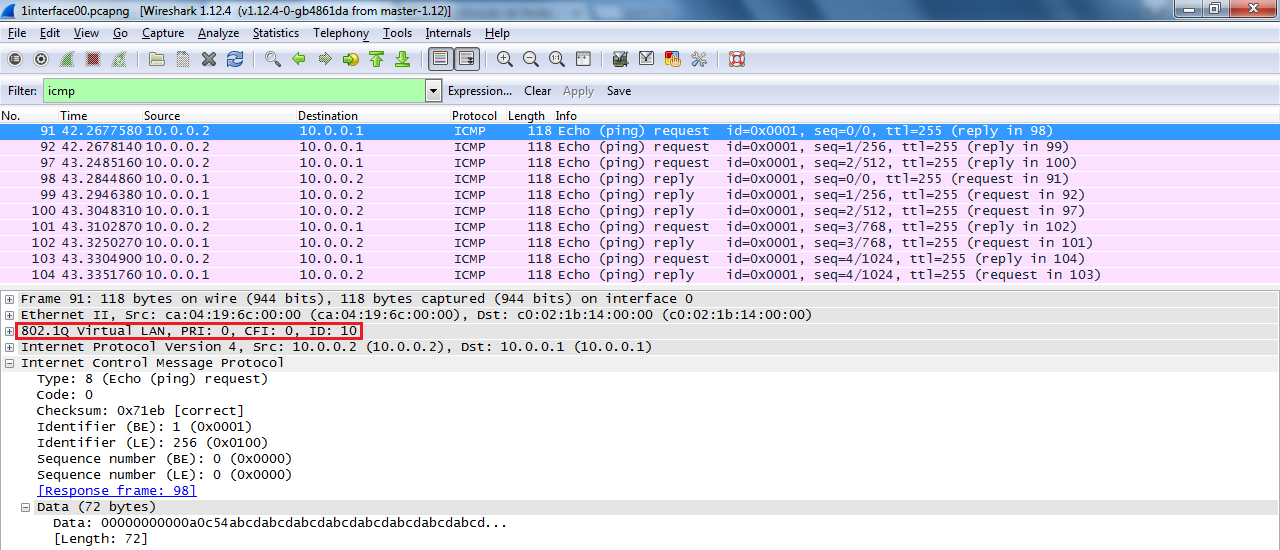
\includegraphics[width=1\textwidth, height=0.32\textheight]{1_interface00-groucho.png}
\label{fig:2-capturaWireshark}
\caption{Captura \emph{wireshark} na interface \textsf{f0/0} de \textsf{groucho}.}
\end{figure}

\begin{figure}[h]
\centering
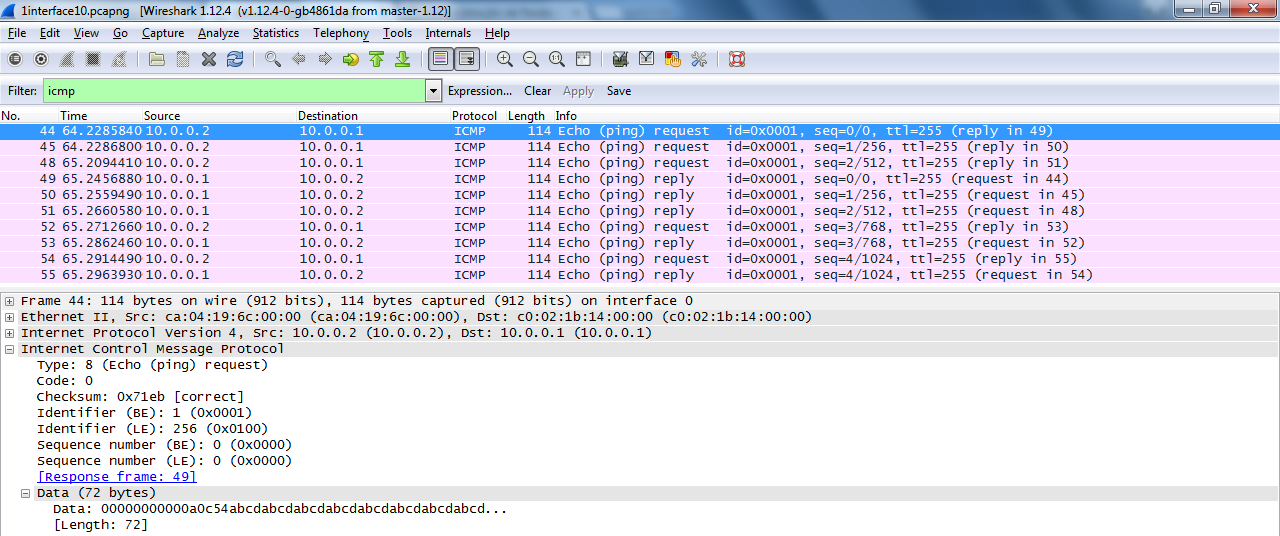
\includegraphics[width=1\textwidth, height=0.32\textheight]{1_interface10-R1.png}
\label{fig:3-capturaWireshark}
\caption{Captura \emph{wireshark} na interface \textsf{f1/0} de \textsf{R1}.}
\end{figure}


\subparagraph{b.}
Quais foram as diferenças encontradas e a que se devem? (texRes)

%no primeiro ICMP \emph{Echo Request} enviado na interface de R1 encontra-se um encapsulamento diferente 802.1Q (portas trunk), ao contrário de na intergace do groucho.


\paragraph{2.}
Na interface \textsf{f1/0} de \textsf{R1} podemos observar que é enviadas várias
mensagens ARP (ARP \emph{Request}) em \emph{Broadcast}, 
(\texttt{Who has 10.0.0.2? Tell 10.0.0.4}), que significa que o \emph{host} 
10.0.0.4 está a tentar descobrir quem é a máquina 10.0.0.2, à qual não se obteve
nenhuma resposta.

Isto acontece porque as portas de \textsf{SW1} estão configuradas em 
\textbf{modo acesso} na VLAN 10 (\textsf{groucho}) e na VLAN20  (\textsf{averell}), 
apesar de ambos os IPs (de \textsf{groucho} e \textsf{averell}) pertencerem à mesma subnet, o \texttt{ping} nunca chega à máquina do \textsf{groucho} (na captura 
\emph{wireshark} na interface \textsf{f0/0} não chega nenhuma mensagem) uma vez que 
as máquinas pertencem a VLANs diferentes.


\paragraph{3.}
 Faça um ping de groucho para averell. O que observa em relação aos pacotes ICMP? (capRes + texRes)
 
\begin{figure}[h]
\centering
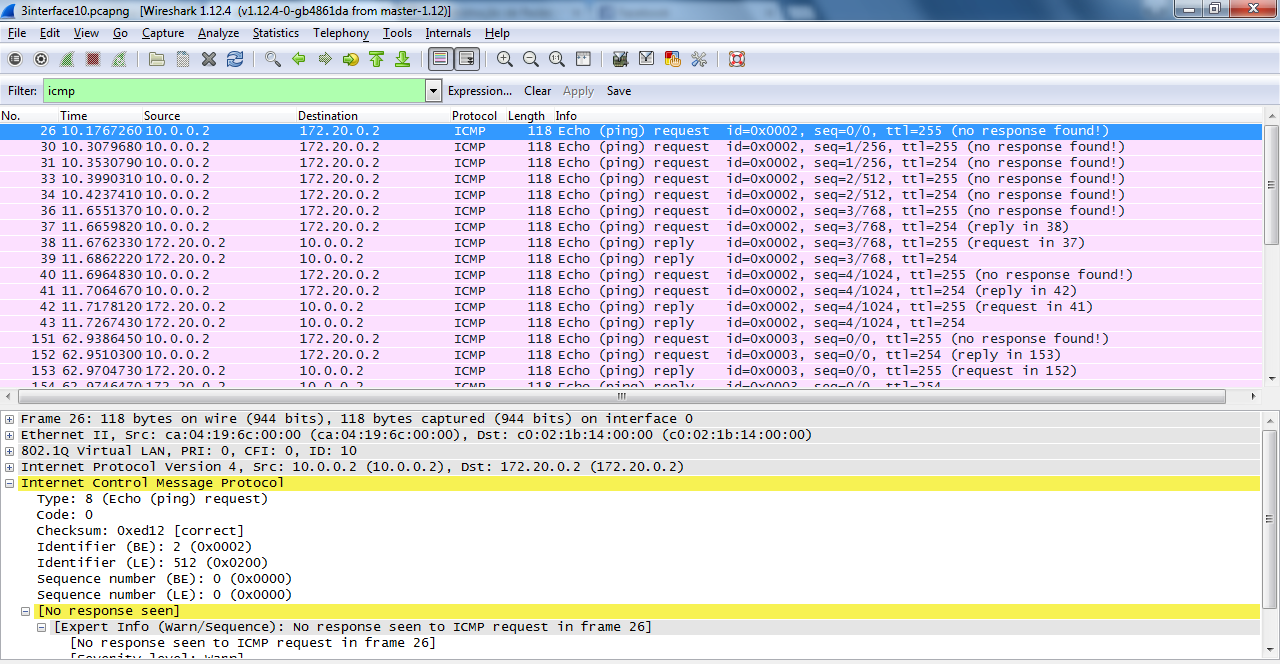
\includegraphics[width=1\textwidth, height=0.38\textheight]{3_interface10_R1.png}
\label{fig:4-capturaWireshark}
\caption{Captura \emph{wireshark} na interface \textsf{f1/0} de \textsf{R1}.}
\end{figure}


\paragraph{4.}

\subparagraph{a.}
Para que a ligação entre \textsf{R1} e o terminal \textsf{linux} funcione em modo \emph{trunk} tivemos de realizar as seguintes configurações.

No \emph{router} \textsf{R1}:
\begin{verbatim}
interface FastEthernet 1/3
switchport trunk encapsulation dot1q
switchport mode trunk
\end{verbatim}

No terminal \textsf{linux}:
\begin{verbatim}
[root@Labs5610 ar]# modprobe 8021q
[root@Labs5610 ar]# vconfig add tap0 10
Added VLAN with VID == 10 to IF -:tap0:-
[root@Labs5610 ar]# 
[root@Labs5610 ar]# ifconfig tap0.10 10.0.0.5 netmask 255.255.255.0 up
\end{verbatim}

\newpage

\subparagraph{b.}
Captura de um pacote do \textsf{ping} (ICMP) enviado em ambas as interfaces:

\begin{figure}[h]
\centering
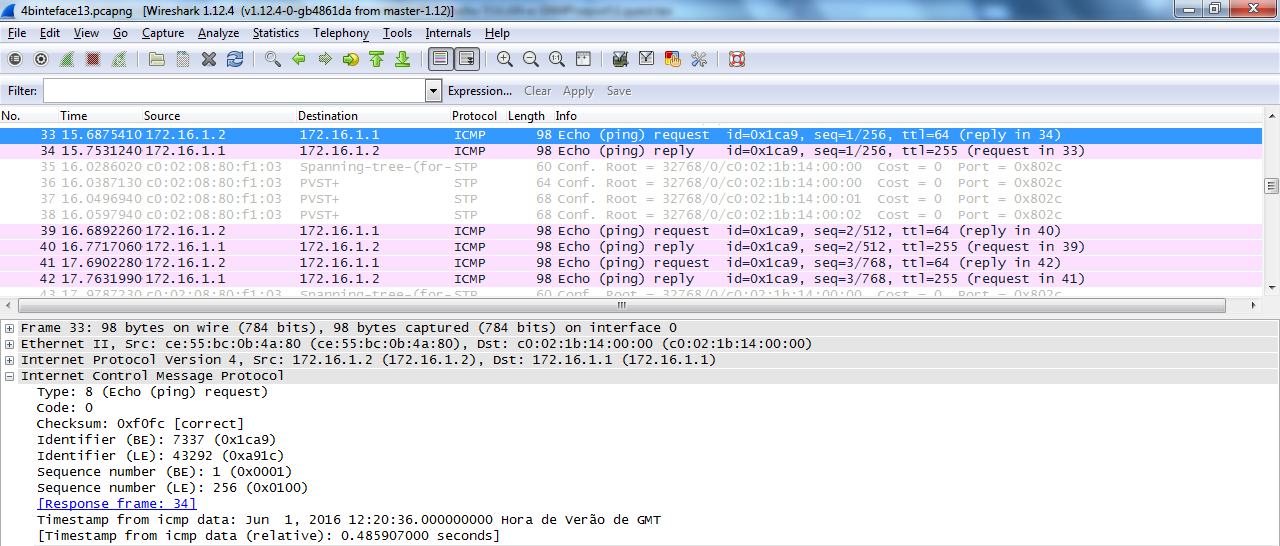
\includegraphics[width=1\textwidth, height=0.32\textheight]{4_ping_VLAN1.png}
\label{fig:5-capturaWireshark}
\caption{Captura \emph{wireshark} de um pacote do \texttt{ping} enviado do terminal \textsf{linux} para a \textsf{VLAN 1}.}
\end{figure}

\begin{figure}[h]
\centering
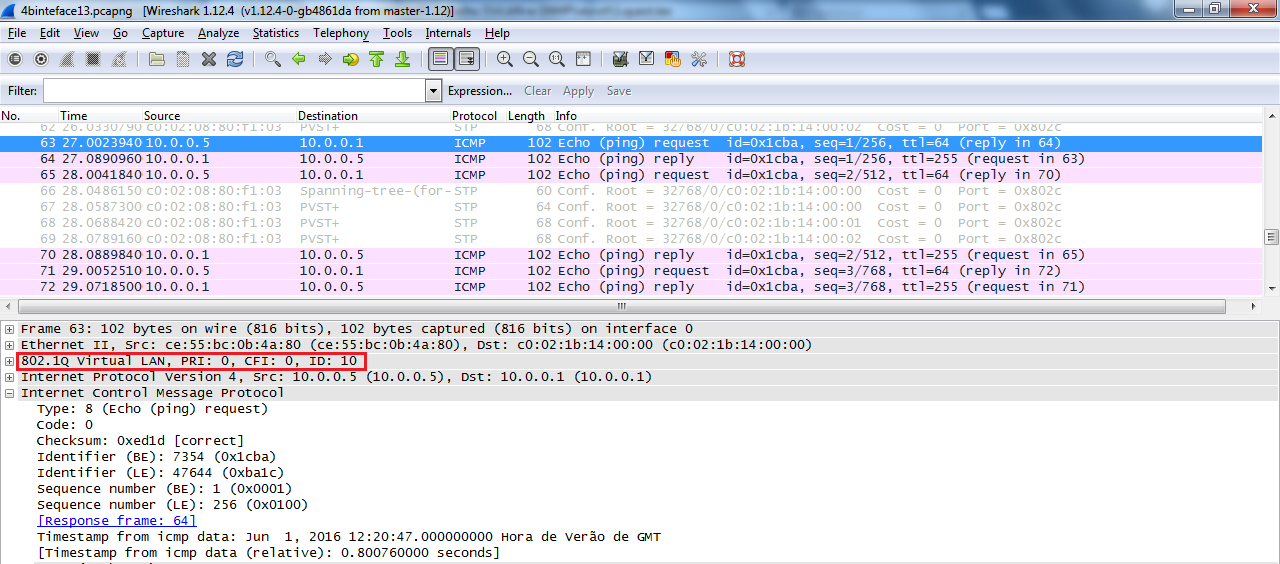
\includegraphics[width=1\textwidth, height=0.32\textheight]{4_ping_VLAN10.png}
\label{fig:6-capturaWireshark}
\caption{Captura \emph{wireshark} de um pacote do \texttt{ping} enviado do terminal \textsf{linux} para a \textsf{VLAN 10}.}
\end{figure}

\newpage

\subparagraph{c.}
Como explica o que observou na alínea anterior? (texRes)


\paragraph{5.}

\subparagraph{a.}
\begin{verbatim}
[root@Labs5610 ar]# snmpget -v 2c -c Leitura 172.16.1.1
 iso.org.dod.internet.mgmt.mib-2.system.sysDescr
SNMPv2-MIB::sysDescr = No Such Instance currently exists at this OID
\end{verbatim}

Não se conseguiu realizar o \texttt{get} porque foi solicitada uma classe e não uma instância.

Quando queremos usar um OID precisamos de adicionar um outro número para obter o valor dessa variável. Por isso, precisamos de acrescentar um \texttt{.0} que representa a primeira instância desse objeto.


\subparagraph{b.}
\begin{verbatim}
[root@Labs5610 ar]# snmpget -v 2c -c Leitura 172.16.1.1
 iso.org.dod.internet.mgmt.mib-2.system.sysDescr.0
SNMPv2-MIB::sysDescr.0 = STRING: Cisco IOS Software, 2600 Software
 (C2691-ADVIPSERVICESK9-M), Version 12.4(15)T6, RELEASE SOFTWARE (fc2)
Technical Support: http://www.cisco.com/techsupport
Copyright (c) 1986-2008 by Cisco Systems, Inc.
Compiled Mon 07-Jul-08 04:30 by prod_rel_team
\end{verbatim}


\subparagraph{c.}
O \texttt{getnext} serve para retornar a instância da classe OID, na árvore de MIB de dados, a seguir à instância descrita no comando. Ou seja, retorna o valor da variável sucessora lexicográfica.


\begin{verbatim}
[root@Labs5610 ar]# snmpgetnext -v 2c -c Leitura 172.16.1.1
 iso.org.dod.internet.mgmt.mib-2.system.sysDescr.0
SNMPv2-MIB::sysObjectID.0 = OID: SNMPv2-SMI::enterprises.9.1.122
\end{verbatim}


\subparagraph{d.}
O \texttt{walk} percorre todas as instâncias de todas as classes respeitando a hierarquia. É construído de  acordo com  as  respostas  que  vai  recebendo  do  \texttt{get-next-request} (ver  na captura abaixo) para recolher a informação a seguir.

Ou seja, o objetivo é recupera uma sub-árvore de valores usando repetidas solicitações SNMP GetNext.

Se é dado um OID, este especifica qual parte do espaço serão pesquisadas usando as solicitações \texttt{getnext}. Todas as variáveis na sub-árvore abaixo desse OID serão consultadas e os seus valores mostrados ao utilizador.

Se não é dados nenhum OID, o \texttt{walk} irá procurar a sub-árvore a partir de SNMPv2-SMI :: mib-2.
O \texttt{walk} para quando retorna resultados que já não estão dentro do alcance do OID.

\begin{figure}[h]
\centering
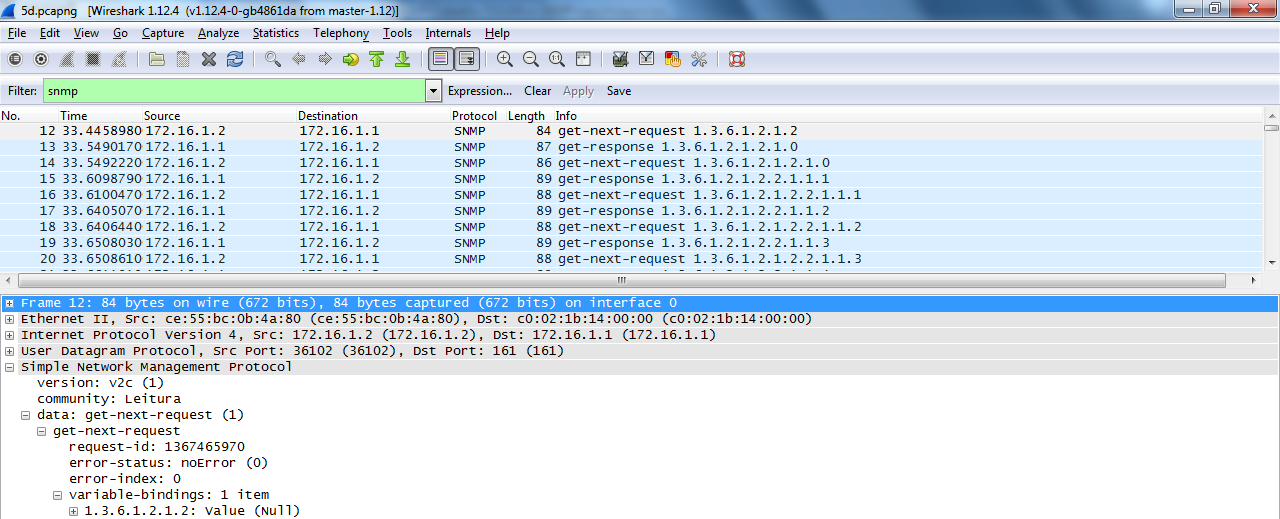
\includegraphics[width=1\textwidth, height=0.3\textheight]{5d.png}
\label{fig:7-capturaWireshark}
\caption{Captura \emph{wireshark} de pacotes SNMP na interface \textsf{f1/3} de \textsf{R1}.}
\end{figure}

\newpage

\subparagraph{e.}
Com base nos resultados da alínea anterior, diga quantas interfaces tem o router e quais são elas. (texRes)

O \emph{router} tem 22 interfaces, que são as que se seguem (parte da resposta do \texttt{snmpwalk} no terminal \textsc{linux}):

\begin{verbatim}
IF-MIB::ifNumber.0 = INTEGER: 22
...
IF-MIB::ifDescr.1 = STRING: FastEthernet0/0
IF-MIB::ifDescr.2 = STRING: FastEthernet0/1
IF-MIB::ifDescr.3 = STRING: FastEthernet1/0
IF-MIB::ifDescr.4 = STRING: FastEthernet1/1
IF-MIB::ifDescr.5 = STRING: FastEthernet1/2
IF-MIB::ifDescr.6 = STRING: FastEthernet1/3
IF-MIB::ifDescr.7 = STRING: FastEthernet1/4
IF-MIB::ifDescr.8 = STRING: FastEthernet1/5
IF-MIB::ifDescr.9 = STRING: FastEthernet1/6
IF-MIB::ifDescr.10 = STRING: FastEthernet1/7
IF-MIB::ifDescr.11 = STRING: FastEthernet1/8
IF-MIB::ifDescr.12 = STRING: FastEthernet1/9
IF-MIB::ifDescr.13 = STRING: FastEthernet1/10
IF-MIB::ifDescr.14 = STRING: FastEthernet1/11
IF-MIB::ifDescr.15 = STRING: FastEthernet1/12
IF-MIB::ifDescr.16 = STRING: FastEthernet1/13
IF-MIB::ifDescr.17 = STRING: FastEthernet1/14
IF-MIB::ifDescr.18 = STRING: FastEthernet1/15
IF-MIB::ifDescr.20 = STRING: Null0
IF-MIB::ifDescr.21 = STRING: Vlan1
IF-MIB::ifDescr.22 = STRING: Vlan10
IF-MIB::ifDescr.23 = STRING: Vlan20
...
\end{verbatim}


\subparagraph{f.}
Resultado do \texttt{get}:
\begin{verbatim}
[root@Labs5610 ar]# snmpget -v 2c -c Leitura 172.16.1.1
 iso.org.dod.internet.mgmt.mib-2.system.sysName.0
SNMPv2-MIB::sysName.0 = STRING: R1
\end{verbatim}

Comando usado para fazer o \texttt{set}:
\begin{verbatim}
[root@Labs5610 ar]# snmpset -v 2c -c Escrita 172.16.1.1
 iso.org.dod.internet.mgmt.mib-2.system.sysName.0 s R2
SNMPv2-MIB::sysName.0 = STRING: R2
\end{verbatim}


\subparagraph{g.}
Faça um walk e um bulkwalk à sub-árvore system da MIB-2. Qual é a diferença entre estes dois comandos e em que se traduz na prática????? (2×capRes + texRes)

O \texttt{bulkwalk} obtém a informação com apenas um pedido, uma vez que usa solicitações SNMP GetBulk (\texttt{get-bulk-request} que permite a transferência de grandes volumes de informação). Enquanto que o \texttt{walk} usa solicitações SNMP GetNext, que realiza um pedido para cada variável, como já foi explicado acima.
A vantagem do \texttt{bulkwalk} em relação ao \texttt{walk} é o ganho em termos de eficiência. Nas capturas a seguir podemos reparar na diferença de quantidade de pedidos  feitos entre os 2, através da barra lateral.


\begin{figure}[h]
\centering
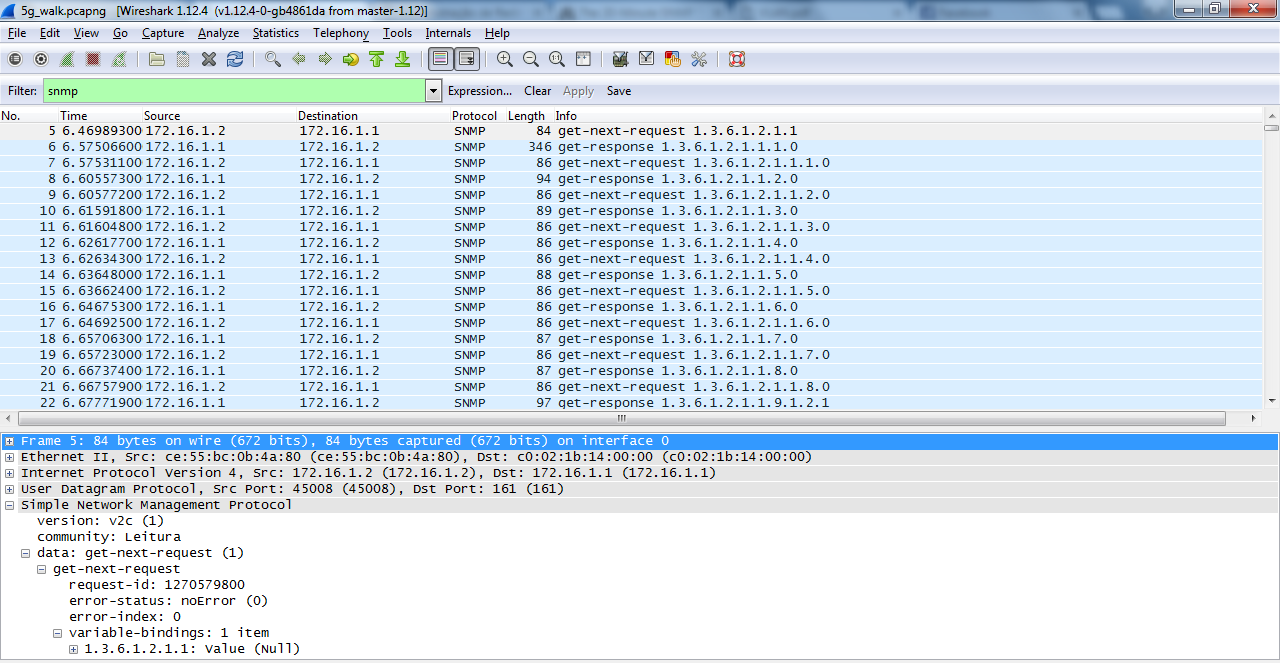
\includegraphics[width=1\textwidth, height=0.35\textheight]{5g_walk.png}
\label{fig:8-capturaWireshark}
\caption{Captura \emph{wireshark} de pacotes \texttt{snmpwalk}.}
\end{figure}

\begin{figure}[h]
\centering
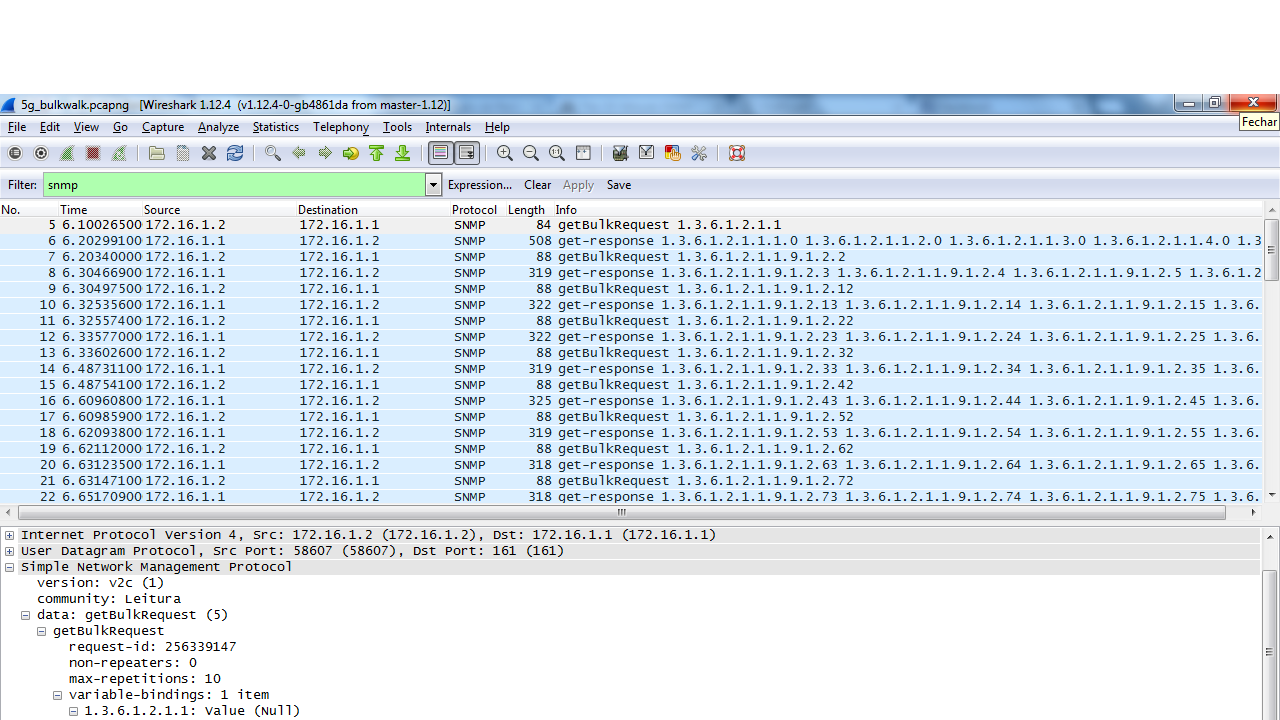
\includegraphics[width=1\textwidth, height=0.4\textheight]{5g_bulkwalk.png}
\label{fig:9-capturaWireshark}
\caption{Captura \emph{wireshark} de pacotes \texttt{bulkwalk}.}
\end{figure}

\newpage

\subparagraph{h.}
Informação sobre as interfaces de \textsf{R1}:
\begin{verbatim}
[root@Labs5610 ar]# snmpnetstat -v 2c -Ci -c Leitura 172.16.1.1
Name      Mtu Network     Address    Ipkts Ierrs Opkts Oerrs Queue
Fa0/0    1500                            0     0     0     0     0
Fa0/1    1500                            0     0     0     0     0
Fa1/0    1500                            0     0     0     0     0
Fa1/1    1500                            0     0     0     0     0
Fa1/2    1500                            0     0     0     0     0
Fa1/3    1500                            0     0     0     0     0
Fa1/4    1500                            0     0     0     0     0
Fa1/5    1500                            0     0     0     0     0
Fa1/6    1500                            0     0     0     0     0
Fa1/7    1500                            0     0     0     0     0
Fa1/8    1500                            0     0     0     0     0
Fa1/9    1500                            0     0     0     0     0
Fa1/10   1500                            0     0     0     0     0
Fa1/11   1500                            0     0     0     0     0
Fa1/12   1500                            0     0     0     0     0
Fa1/13   1500                            0     0     0     0     0
Fa1/14   1500                            0     0     0     0     0
Fa1/15   1500                            0     0     0     0     0
Nu0      1500                            0     0     0     0     0
Vl1      1500 172.16.1/24 172.16.1.1  1178     0  1183     0     0
Vl10     1500 10.0.0/24   10.0.0.1      61     0    39     0     0
Vl20     1500 172.20.0/24 172.20.0.1    47     0    29     0     0
\end{verbatim}

\newpage

Informação sobre a tabela de encaminhamento de \textsf{R1}:
\begin{verbatim}
[root@Labs5610 ar]# snmpnetstat -v 2c -Cr -c Leitura 172.16.1.1
Routing tables (ipCidrRouteTable)
Destination                Gateway            Flags   Interface
10.0.0/24                  *                  <U>     Vl10
172.16.1/24                *                  <U>     Vl1
172.20.0/24                *                  <U>     Vl20
\end{verbatim}


\paragraph{6.}

\subparagraph{a.}
Tabela de informação sobre os endereços IP de \textsf{R1}:
\begin{verbatim}
[root@Labs5610 ar]# snmptable -v 2c -c Leitura 172.16.1.1 ip.ipAddrTable
SNMP table: IP-MIB::ipAddrTable

 ipAdEntAddr ipAdEntIfIndex ipAdEntNetMask ipAdEntBcastAddr ipAdEntReasmMaxSize
    10.0.0.1             22  255.255.255.0                1               18024
  172.16.1.1             21  255.255.255.0                1               18024
  172.20.0.1             23  255.255.255.0                1               18024

\end{verbatim}


\subparagraph{b.}
Com base na sua definição no módulo IP-MIB, explique o que faz com que ip.ipAddrTable seja uma tabela. (texRes)


\subparagraph{c.}
Diga como se mapeiam as linhas (índices) e as colunas de uma tabela em OIDs na estrutura em árvore da MIB. (texRes)

Para mapear tabelas na estrutura em árvore é necessário definir parte da MIB como tabular e mapear a linha e a coluna da tabela no OID que contém a respetiva entrada.

É de notar que, a coluna pode ser sempre identificada por um número (número da coluna), a linha é identificada pelo índice, e que no mapeamento para o OID, aparece primeiro a coluna e depois  a linha.


\paragraph{7.}

\subparagraph{a.}
Na captura podemos observar que é enviado um \emph{trap} a informar de uma \emph{generic-trap: linkDown}, relativa à falha da ligação da interface \textsf{f1/2}.

No terminal \textsf{linux} podemos ver a receção desse \emph{trap}:
\begin{verbatim}
[root@Labs5610 ar]# snmptrapd -n -f -Lo
NET-SNMP version 5.7.3
2016-06-02 10:38:04 172.16.1.1(via UDP: [172.16.1.1]:62413->[172.16.1.2]:162)
 TRAP, SNMP v1, community traps7
	SNMPv2-MIB::snmpTraps Link Down Trap (0) Uptime: 0:27:01.63
	IF-MIB::ifIndex.5 = INTEGER: 5	IF-MIB::ifDescr.5 = STRING: FastEthernet1/2
	IF-MIB::ifType.5 = INTEGER: ethernetCsmacd(6)	
	SNMPv2-SMI::enterprises.9.2.2.1.1.20.5 = STRING: "administratively down"
\end{verbatim}

Onde podemos ver que é informado que a ligação da interface \textsf{f1/2} (\texttt{IF-MIB::ifDescr.5 = STRING: FastEthernet1/2}) é desativada administrativamente ( a string \texttt{SNMPv2-SMI::enterprises.9.2.2.1.1.20.5} foi alterada para \texttt{"administratively down"}).

\begin{figure}[h]
\centering
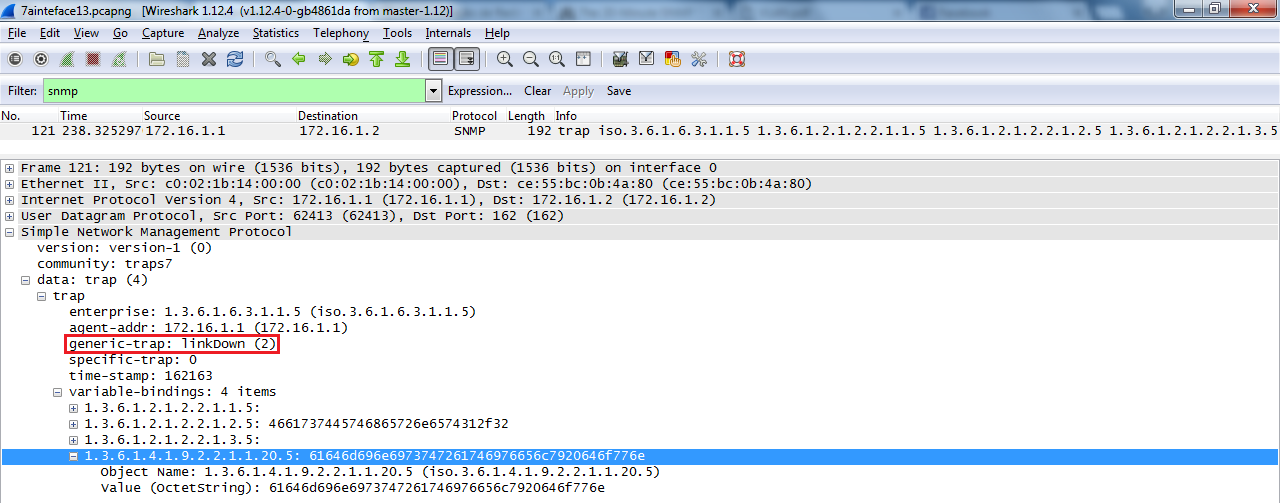
\includegraphics[width=1\textwidth, height=0.3\textheight]{7a.png}
\label{fig:10-capturaWireshark}
\caption{Captura \emph{wireshark} na interface \textsf{1/3} de \textsf{R1}.}
\end{figure}

\newpage

\subparagraph{b.}
Captura de pacotes SNMP na interface \textsf{f1/3} de \textsf{R1}:

\begin{figure}[h]
\centering
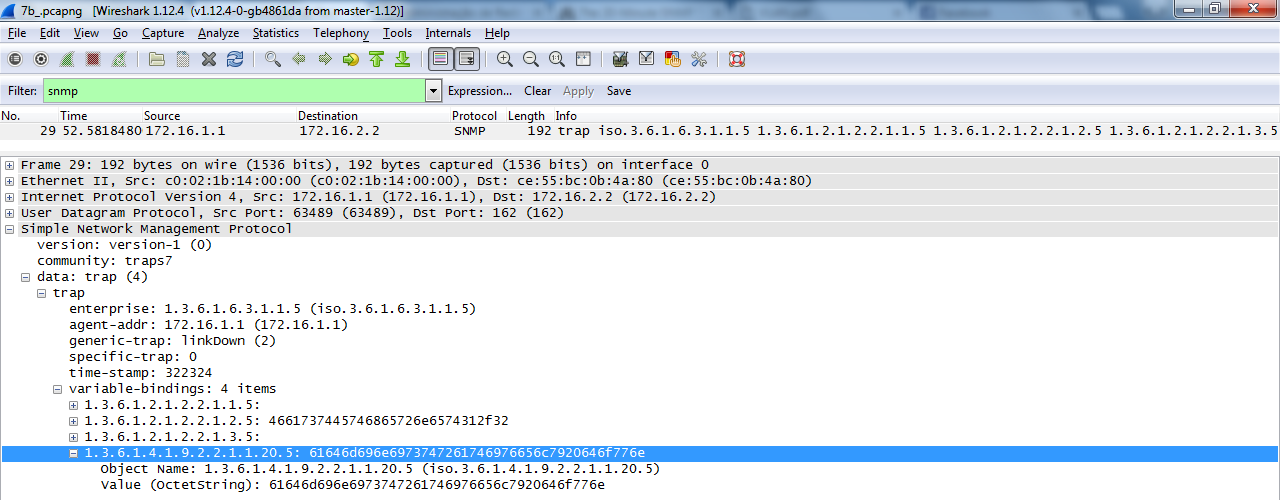
\includegraphics[width=1\textwidth, height=0.3\textheight]{7b.png}
\label{fig:11-capturaWireshark}
\caption{Captura \emph{wireshark} na interface \textsf{1/3} de \textsf{R1}.}
\end{figure}

\newpage

\subparagraph{c.}
Captura de pacotes SNMP na interface \textsf{f1/3} de \textsf{R1}:

\begin{figure}[h]
\centering
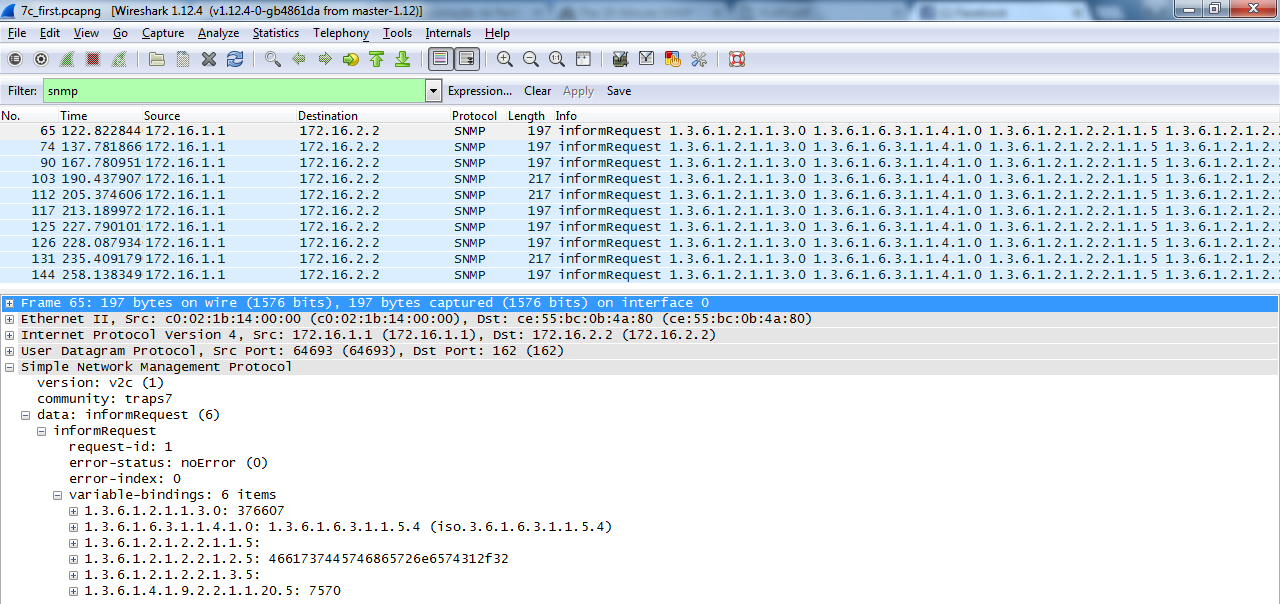
\includegraphics[width=1\textwidth, height=0.33\textheight]{7c.png}
\label{fig:12-capturaWireshark}
\caption{Captura \emph{wireshark} na interface \textsf{1/3} de \textsf{R1}.}
\end{figure}


\subparagraph{d.}
Captura de pacotes SNMP na interface \textsf{f1/3} de \textsf{R1}:

\begin{figure}[h]
\centering
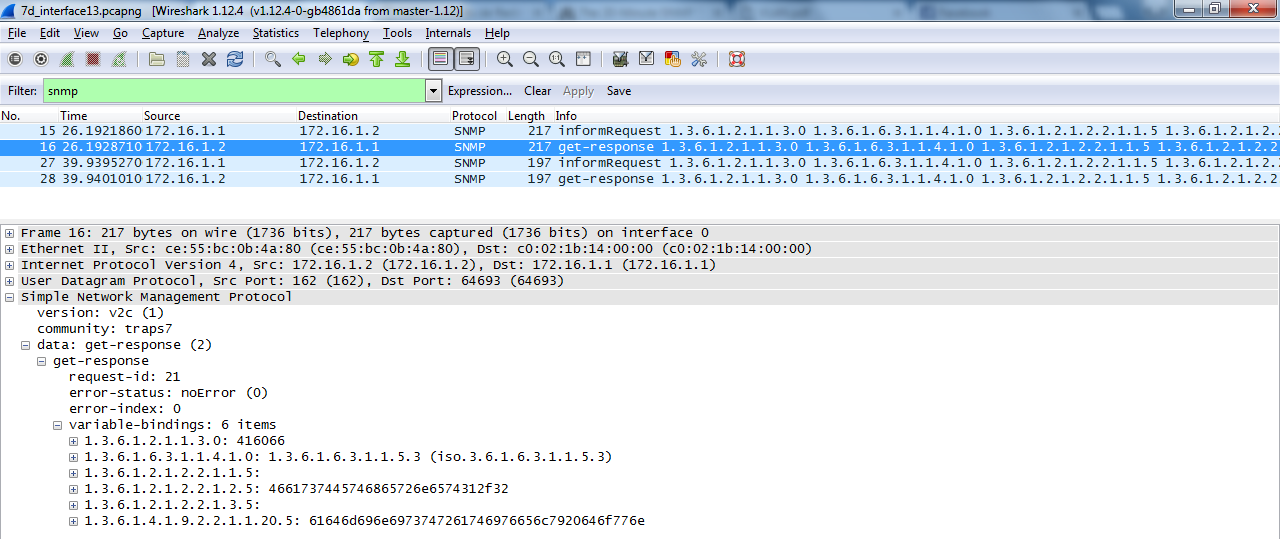
\includegraphics[width=1\textwidth, height=0.3\textheight]{7d.png}
\label{fig:13-capturaWireshark}
\caption{Captura \emph{wireshark} na interface \textsf{1/3} de \textsf{R1}.}
\end{figure}


\subparagraph{e.}
Com base nas alíneas anteriores, comente as diferenças entre o uso de informs e de traps, bem como as implicações práticas???? dessas diferenças. (texRes)

\emph{traps} servem para notificar, de forma assíncrona, o gestor da ocorrência de um dado evento, aqui as mensagens não são confirmadas, o que implica uma entrega não-fiável. Em reação à receção de uma \emph{trap}, o gestor pode fazer pedidos para
obter mais variáveis que lhe dêem informação adicional.

\emph{informs} são semelhantes à \emph{trap}, mas com receção confirmada. São concebidos para comunicação entre gestores, mas pode também ser enviados por um agente a um gestor.


\paragraph{8.}

\subparagraph{a.}
Captura dos pacotes trocados quando executados os seguintes comandos:

\begin{itemize}

\item \texttt{snmpgetnext -v2c -c Leitura 172.16.1.1 system.sysName}:

\begin{figure}[h]
\centering
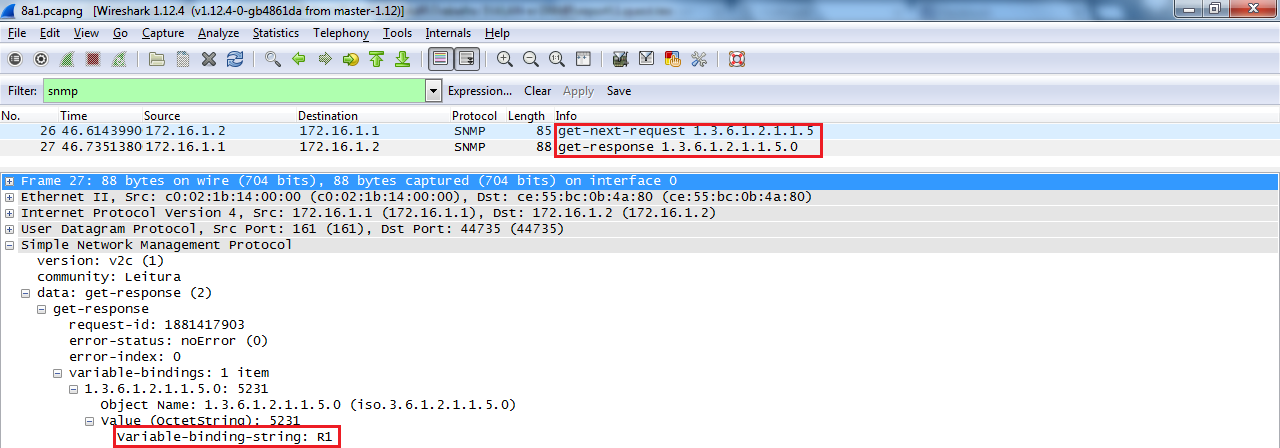
\includegraphics[width=1\textwidth, height=0.28\textheight]{8a1.png}
\label{fig:14-capturaWireshark}
\caption{Captura \emph{wireshark} na interface \textsf{1/3} de \textsf{R1}.}
\end{figure}


\item \texttt{snmpgetnext -v3 -l authNoPriv -u grupo11 -a md5 -A passlimi 172.16.1.1 system.sysName}:

\begin{figure}[h]
\centering
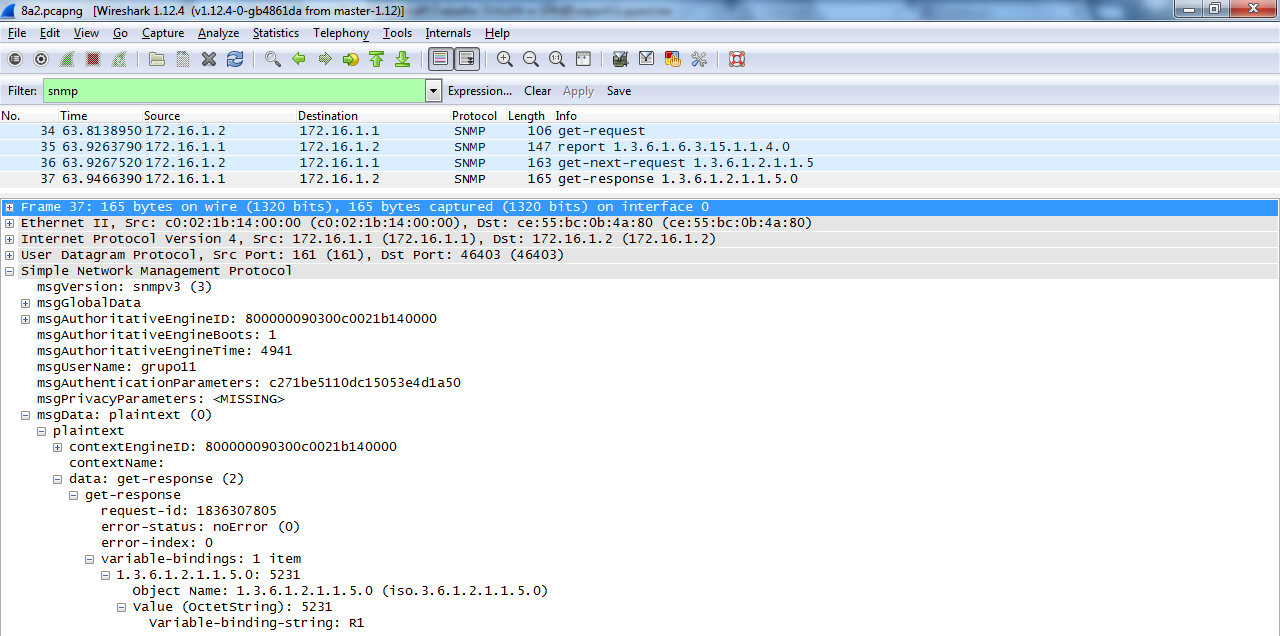
\includegraphics[width=1\textwidth, height=0.35\textheight]{8a2.png}
\label{fig:15-capturaWireshark}
\caption{Captura \emph{wireshark} na interface \textsf{1/3} de \textsf{R1}.}
\end{figure}


\item \texttt{snmpgetnext -v3 -l authPriv -u cifragrupo11 -a md5 -A passlimi -x des -X cifralimi 172.16.1.1 system.sysName}:

\begin{figure}[h]
\centering
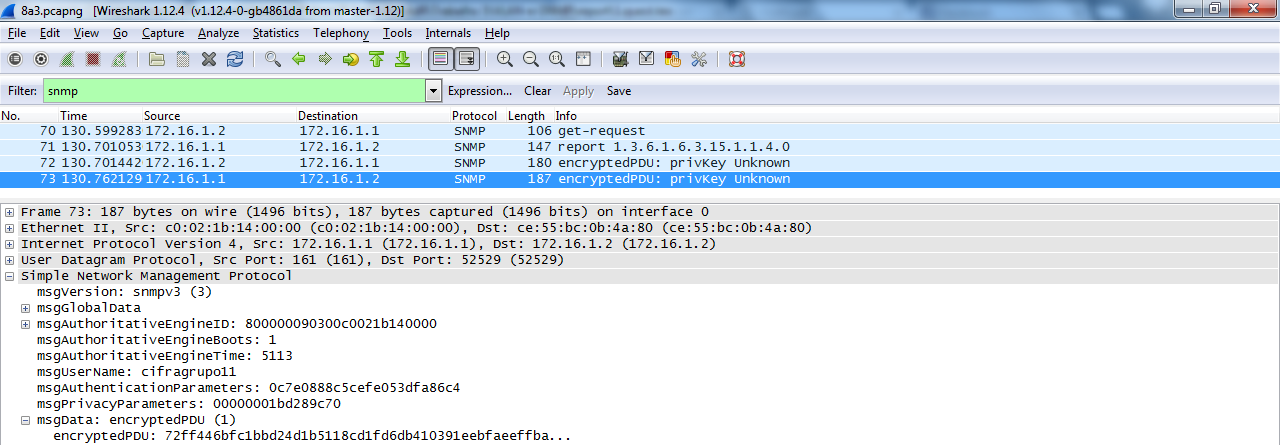
\includegraphics[width=1\textwidth, height=0.3\textheight]{8a3.png}
\label{fig:16-capturaWireshark}
\caption{Captura \emph{wireshark} na interface \textsf{1/3} de \textsf{R1}.}
\end{figure}

\end{itemize}


\subparagraph{b.}
A segurança em SNMPv2 é baseada em autenticação por \emph{strings} de comunicação, uma espécie de \emph{password} partilhada que circula em \emph{clear text}, sendo este o caso menos seguro.

O SNMPv3 suporta autenticação segura, recorrendo a \emph{hashes} criptográficos, também permite definir diferentes níveis de acesso a diferentes partes da MIB para diferentes utilizadores, e suporta garantia de integridade das mensagens.
Este possui 3 níveis de segurança, \textsf{noAuthNoPriv}, \textsf{AuthNoPriv} e \textsf{AuthPriv}, sendo os dois últimos experimentados neste trabalho.

Podemos afirmar que o nível de segurança \textsf{AuthPriv} é mais seguro de que o \textsf{AuthNoPriv}, uma vez que ele suporta cifragem das mensagens de modo a garantir privacidade, ao contrário do nível de segurança \textsf{AuthNoPriv}.